\section{Introduction}~\label{sec:introduction}

\todo{Spiel about reversible computing and logical reversibility}

\todo{Spiel about 2-categorical view of PLs, classical languages are (2,1), reversible languages are (2,0)}

\subsection*{Outline and Contributions}

\begin{itemize}[leftmargin=*]
\item We take the $\PiLang$ family of reversible languages~\cite{jamesInformationEffects2012} and show how to encode various boolean reversible circuits in the language. The circuits are implemented using 1-combinators in the language, and circuit optimisations are realised as 2-combinators between these reversible programs.
\item We show how to encode reversible circuits on a fixed number of bits as permutations of finite sets with the appropriate cardinality. We observe that reversible programs can be translated to bijective functions between finite sets and equality of reversible programs can be witnessed as extensional equality of these bijective functions, which is decidable.
\item We review a few basics of Homotopy Type Theory~\cite{univalentfoundationsprogramHomotopyTypeTheory2013}, and exhibit some results that we use in our technical development. We define the notion of a universe \`{a} la Tarski internally in HoTT, which is given by a type for codes $U$ and a decoding function to a univalent universe $\El : U \to \UU$. We say that this universe is univalent, if the decoding fibration is univalent, that is, the decoding function $\El$ reflects the path space of the underlying univalent universe. We exhibit some examples of univalent subuniverses, in particular, we define the subuniverse of finite types, $\UFin$, which classifies all types with a specified cardinality $n : \Nat$, and show that it is univalent. Hence, we establish a characterisation of the path space of the universe of finite types.
\item We observe that 1-paths in $\UFin$ are permutations on finite sets with a fixed cardinality $n$, given by $\Aut[\Fin[n]]$. We define Lehmer codes~\cite{lehmerTeachingCombinatorialTricks1960} for permutations, which are a convenient and compact representation of permutations. We show that there is an equivalence between Lehmer codes and permutations $\Lehmer[n] \eqv \Aut[\Fin[n]]$ given by the Lehmer encode-decode algorithm.
\item Then, we give a presentation of the symmetric group $\Sn[n]$ on $n$ generators, given by the set-quotient of $\List[\Fin[n]]$ by Coxeter relations. We define the short form and long form of the Coxeter relations for the symmetric group, and show that the long form of the relation is (locally) confluent and strongly normalising, and that both the forms are equivalent. From this, we show that the Coxeter relation produces a normal form for words in $\Sn$. We further show that this indeed gives a group presentation for $\Sn$, and that we can decode a Lehmer code to a word in $\Sn[n]$ and back, giving the equivalence $\Sn[n] \eqv \Lehmer[n]$. This gives an axiomatisation of permutations on $\Fin[n]$ as relations on $\List[Fin[n]]$, which we use to interpret our language $\PiLang$ in our model.
\item Then, we show that $\UFin$ has a symmetric monoidal structure (the additive one), where the unit is given by the empty set, and the tensor product of two finite sets is given by their disjoint union. We show that this satisfies the associator, unitor and symmetry isomorphisms of a symmetric monoidal category, and Mac Lane's pentagon, hexagon, and syllepsis coherence conditions. This gives a complete characterisation of our model $\UFin$ which we interpret our language $\PiLang$ into.
\item Finally, we interpret the language $\PiLang$ into our model. First we define a subset of the language $\PiPlusLang$ which only includes the additive monoidal structure. Then, we define a normalised form for this language in $\PiHatLang$, where the objects of the language are simply the unary natural numbers, and give normalised 1-combinators and 2-combinators which perform adjacent transpositions.
\item We show how to interpret this language $\PiHatLang$ into $\UFin$, translating the natural numbers into the cardinality of the finite set, 1-combinators into permutations via words in $\Sn$, and 2-combinators as 2-paths in $\UFin$. We further show how to quote back a permutation in $\UFin$ into a 1-combinator using the normal form for words in $\Sn$. We show that this gives a symmetric monoidal equivalence.
\item Then, we show that $\PiPlusLang$ can be translated into $\PiHatLang$. The 1-combinators are translated as composition of adjacent transpositions, and the 2-combinators are interpreted using the coherence conditions for symmetric monoidal categories. We further show that this translation can be inverted, giving a symmetric monoidal equivalence.
\item Finally, we give a translation from $\PiLang$ to $\PiHatLang$ and $\PiLang$, using the additive structure and distributivity to build the multiplicative structure. We show that this translation reflects 2-combinators. We give some applications of this translation by showing how to normalise a circuit written in $\PiLang$ to a normal form in $\PiPlusLang$ and $\PiHatLang$, which uses fewer gates.
\end{itemize}

Our results are formalised in the proof assistant Agda using the HoTT-Agda library.

\note{Novel interpretation of the univalence axiom, operational and denotational semantics and adequacy.}

\begin{center}
  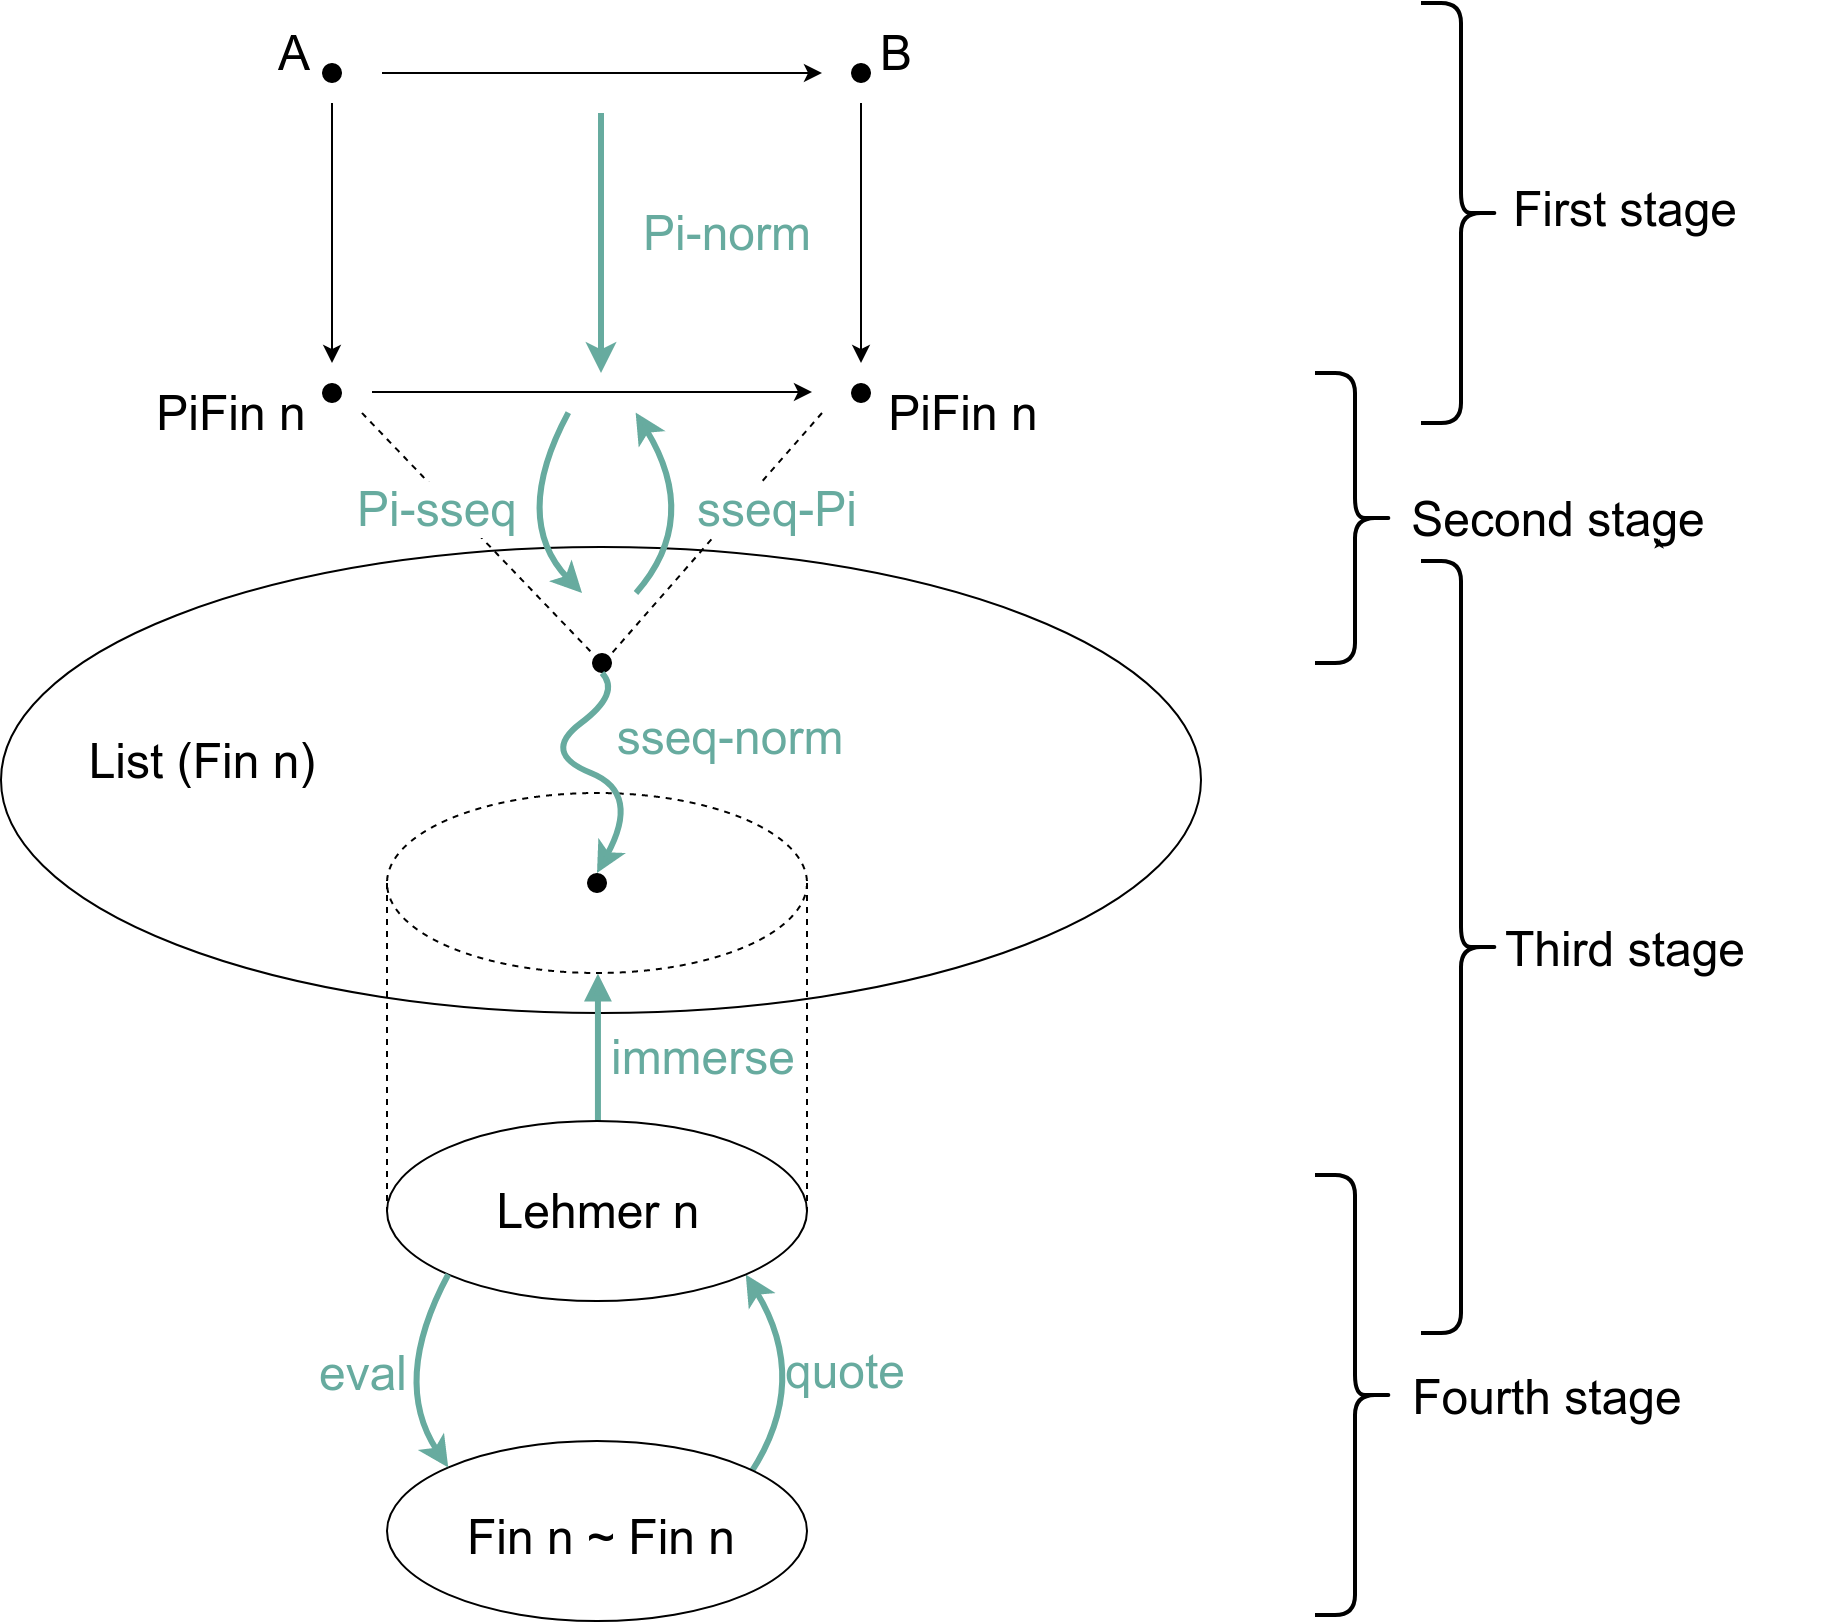
\includegraphics[scale=0.3]{outline.png}
\end{center}


%%% Local Variables:
%%% mode: latex
%%% TeX-master: "main"
%%% fill-column: 120
%%% End:
